\chapter{内额皮层:基于输出结果选择动作}

这本书提出了关于灵长类动物前额叶皮层基本功能的方案。
\begin{document}
\section{概述}
内侧PF皮层有助于根据这些动作之前的行为结果来评估和选择动作,其连接指纹解释了它是如何做到这一点的。海马连接提供有关导航和其他涉及动作的事件的信息,杏仁核提供基于当前生物需求的预测结果的最新评估,并且与内侧前运动区域的连接提供了行动的途径。这些与行动和动机有关的“内部”信号与感官输入等外部信号形成对比。中间PF区域基于这些内部因素对行动的选择产生偏见,包括努力成本、更新的估值、预测结果对觅食选择的影响,以及使用内在与外在坐标系来指导行动。在灵长类动物中,内侧PF皮层的颗粒部分通过在反馈时间评估自我产生的选择、平衡竞争性任务规则以及根据单个先前事件做出选择来阐述这些“内部”影响。

\section{介绍}
第一章解释了连接限制了PF皮层的功能。由于其连接因区域而异,本章开始对PF皮层进行区域探索。我们从内侧PF皮层开始,部分原因是它包括PF皮层的一些旧部分(第2章)。\par
第2章区分了内侧PF皮层的颗粒和无颗粒部分,后者在所有哺乳动物中共享。因此,我们想比较大鼠和猴子的无颗粒PF区域。不幸的是,对猴子的这些区域知之甚少。因此,我们被迫依赖啮齿动物(主要是大鼠)的数据。我们认识到这种方法的危险 - 啮齿动物和灵长类动物的最后共同祖先生活在~70-90 Ma,从那以后这两个谱系就分开进化了。这一事实意味着,随着两组动物的进化,两组动物的无颗粒PF区域的连接和功能将发生变化。未来的研究将表明这种差异的程度,但现在我们必须利用我们所拥有的东西来凑合。\par
在灵长类动物中,内侧PF皮层位于内侧前运动区域的喙部,包括前SMA,SMA和CMA(见缩写列表)。帕辛汉姆等(2010)认为,所有这些中间领域都显示出指导和分析基于“内部”信号的行动的专业化。“内部”一词,在这里使用的意义上,是指传达内部状态和记忆的信号,与视觉、听觉、嗅觉、味觉和触觉等外部信号形成鲜明对比。

\section{区域}
图3.1显示了猴子和人类中被指定为内侧PF皮层的区域,图2.1显示了其在猴子,人类和大鼠中的细分视图。在灵长类动物中,内侧PF皮层的颗粒部分由前扣带皮层(区域24),边缘前皮层(主要是区域32)和边缘下皮层(区域25)组成。正如第2章所解释的,所有哺乳动物,包括啮齿动物和灵长类动物,都有这三个区域的同系物。\par
内侧PF皮层的颗粒部分包括区域9的内侧部分和所有区域10,只有灵长类动物有这些区域。第1章证明将极地包括在内是合理的PF皮层(区域10)在内侧区域组,部分基于连接。注意我们将所有极性PF皮层(区域10)都包括在周一的内侧PF皮层内键,但只是它在人类中的内侧部分。
\begin{figure}[!htb]
	\centering
	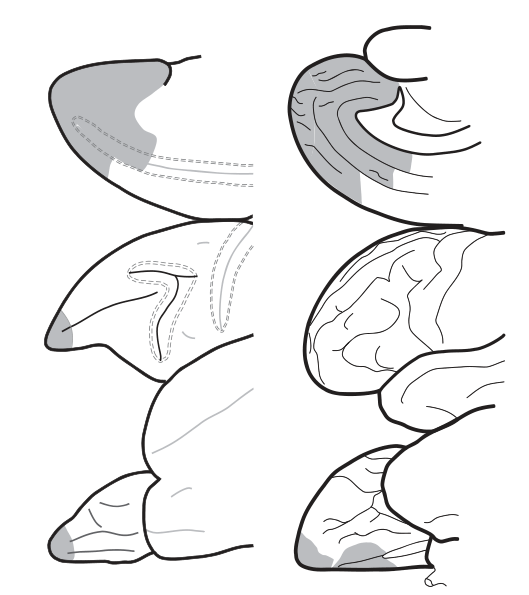
\includegraphics{Fig_3_1}
	\caption*{图3.1 猕猴(左)和人类(右)的内侧PF皮层,用阴影表示。格式如图1.2所示。}
\end{figure}

术语前扣带皮层在文献中有很多含义。在这本书中,我们将边缘前皮层和边缘下皮层排除在我们称为前扣带皮层(图2.1)。我们还排除了扣带运动区域,这些区域我们认为是前运动皮层的一部分。因此,读者应该意识到当我们使用短语 前扣带皮层 ,我们仅指区域 24 的一部分,而不是到运动前区域或内侧PF皮层的其他颗粒状部分。\par
在我们排除在前扣带皮层之外的区域中,眶前和边缘下皮层占据了大部分的眶前和眶下皮层。术语膝下皮层是指胼胝体膝腹侧的皮层,术语膝前皮层是指位于膝侧的无核区域。孕皮质不包括位于更前列的颗粒区域,例如极性PF皮质的内侧部分(区域10)。最后,我们称之为腹内侧PF皮层的14区的状态仍不确定。一些专家将其纳入内侧PF皮层,另一些专家则将其视为眼眶PF皮层的最内侧部分。我们不需要在这些分类之间做出决定,但在大多数情况下,我们保留了第4章关于眼眶PF皮层的区域14的考虑。\par

\section{关系}
图3.2显示了猕猴内侧PF皮层的主要连接。
这个情节和第4-7章中的类似情节旨在传达神经解剖学文献中出现的最重要的概念点。我们不打算提供一个全面的总结,也不关心指出哪些神经解剖学家首先描述了一个特定的途径。这些情节起到了连接指纹的作用,第一章对此进行了解释。连接指纹强调区分PF皮层区域彼此和其他皮层区域的特征,就像人类指纹区分人与人一样。\par
1.海马体和下托与内侧PF皮层的边缘下和边缘前区域有密集的相互连接(Insausti和Muñoz 2001)。海马体和内侧PF皮层之间的间接连接包括前扣带皮层(区域24)和内侧颗粒区域9和10,其中一些通过脾后皮层运行(Kobayashi和Amaral 2003)。内嗅皮层和海马旁皮层也与内侧PF皮层有联系(Kondo等人)\par
2.2003 ; Muñoz和Insausti(2005年)。海马体和内侧PF皮层之间的皮质下通路包括通过乳头体和丘脑的中继。我们认为与海马体的联系对内侧PF皮层的功能特别重要。其他PF区域,如外侧OFC,要么缺乏与海马体的连接,要么具有非常弱的连接(Carmichael和Price 1995a)。稍后,我们解释了我们的观点,即海马体为PF皮层提供了有关导航和其他涉及动作的过去事件的信息。2.内侧PF皮层与杏仁核有着紧密的联系,图3.3显示,这些投射中密度最大的涉及PF皮层的无核部分\par
\begin{figure}[!htb]
	\centering
	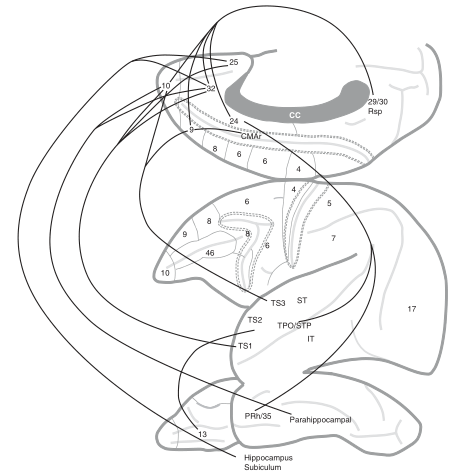
\includegraphics{Fig_3_2}
	\caption*{图3.2猕猴内侧PF皮层的选定连接。图1.4和1.5给出了沟和区域的名称。线连接着一些有直接轴突连接的区域,除非另有说明,否则假设是相互的。}
\end{figure}
(Prather等人,2001年;Morecraft等人,2007年)。颗粒区域,如13m区域,也接受杏仁核输入,图3.3没有说明(Saleem等人,2008年)\par
杏仁核通常被视为在情绪、动机和奖励中发挥作用,包括恐惧调节和对社会刺激(如人脸)的情绪反应。但它在奖励中的作用并不是一般的。双侧杏仁核损伤后,条件性视运动学习完全正常进行,尽管这取决于学习与奖励的关系(Murray和Wise 1996)。因此,奖赏处理本身不能作为杏仁核功能的一般或完整描述。相反,最有力的证据表明,杏仁核和皮层之间的相互作用会根据当前的需求更新结果评估(Baxter和Murray,2002年)。在整本书中,我们使用结果一词来指代以下反馈\par
\begin{figure}[!htb]
	\centering
	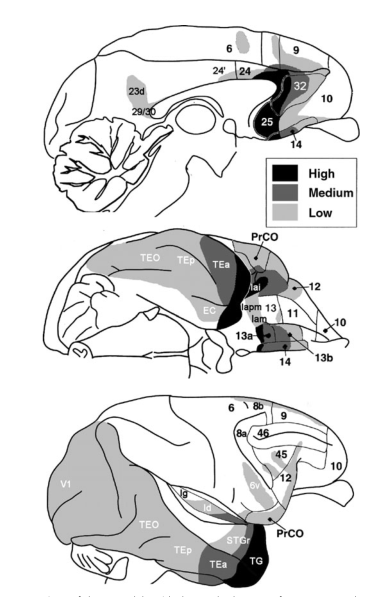
\includegraphics{Fig_3_3}
	\caption*{图3.3猕猴杏仁核与大脑皮层的连接。阴影表示投射的主观密度,重点是从杏仁核到皮层的投射。皮层通常也会发送一个返回投影。缩写:EC,内嗅皮层;Iai、Iapm和Iam,分别为无核岛状区、下分区、后内侧分区和内侧分区;Ig,颗粒状岛叶皮层;Id,粒状岛叶皮层;中央前顶盖皮质;颞上回;TEa、TEp、TEO、颞下区、前部、后部和枕部;TG,颞极皮层;V1,初级视觉(纹状体)皮层(17区)。经麦克米伦出版有限公司(Macmillan Publishers Ltd.)普莱斯·JL(Price JL)、德雷维茨·WC(Drevets WC)许可转载。《情绪障碍的神经回路》,《神经精神药理学》35:192–216,©2009,自然出版集团}
\end{figure}
一种行动,无论是从发生的事情还是在任何特定时间的价值来看。当然,目前的需求不仅涉及营养和液体,还涉及避免伤害和其他生物成本和收益。因此,我们可以说杏仁核有助于评估积极和消极的结果。\par
3.内侧PF皮层直接或间接投射到运动前区域。颗粒内侧PF皮层(9区)与内侧PF皮层的其他部分有联系,特别是与前扣带皮层有联系(Vogt和Pandya 1987)。该区域反过来与前扣带运动区(CMAr)相连,CMAr是内侧前运动皮层的一部分(Morecraft和Van Hoesen,1998)。CMAr位于扣带沟(Dum和Strick,2002年),位于与之相连的术前运动区(preSMA)的腹侧(Luppino等人,1993年)。SMA本身也与尾扣带运动区相互连接(Luppino等人,1993年)。扣带运动区或前SMA和SMA的损伤损害了猴子在没有外部(感觉)提示的情况下做出的运动的产生(Thaler等人,1995年)。因此,我们可以将这些行动称为“内部”指导\par
4.与腹侧PF皮层和眶侧PF皮层不同,内侧PF皮层不接收来自颞下皮层的视觉输入(Carmichael和Price 1995b;Kondo等人2005)。然而,前扣带皮层与嗅周皮层有一些联系,它也接收来自颞上沟TPO区域的输入(Kondo等人,2005年),该区域处理视觉和听觉信息。尽管有这些输入,内侧PF皮层和视觉区域之间的联系并不是特别突出。\par
5.内侧PF皮层,尤其是极性PF皮层(区域10),接收来自颞上皮层的投射,其中大部分来自其吻部,包括颞极(Barbas等人1999;Kondo等人2003)\par
这些投射中一些更尾部的涉及生理学研究表明是听觉的区域(Hackett et al 1998),但其他投射的功能,如靠近颞极的投射,仍然未知\par
6.与PF皮层的许多其他部分不同,内侧PF皮层也投射到下丘脑(Rempel-Clower和Barbas,1998年),以及在内脏运动功能中发挥作用的脑干网状核(Öngür等人,1998年;Barbas等人,2003年)\par
其中一些投射可能会影响自主神经系统,以及大脑控制身体的其他方式。例如,下丘脑外侧调节自主神经的唤醒,下丘脑的室旁核控制神经内分泌和神经分泌的输出。\par
\subsection{总结}
内侧PF皮层的连接指纹表明以下要点:(1)与PF皮层的其他部分相比,内侧PF皮层接收的感觉输入很少;(2) 它与运动前区域相连,该运动前区域在动物蓄能器网络71缺乏来自任何外部线索的动作提示时控制动作;(3)它与海马体和杏仁核有着密切的联系,这表明它既可以获得过去事件的记忆,也可以获得从当前生物需求来看有价值的结果信息\par
尽管这里列出的连接并不总是涉及内侧PF皮层的相同部分,但不同部分相互连接(Barbas 2000),这意味着一个部分的输入可以影响其他部分。第8章将这一观点扩展到整个PF皮层。\par
\section{决策、选择和目标}
尽管“决定”一词可以应用于动物所做的大多数事情,但我们使用这个词的方式更为有限。我们将决策与这些决策之后可能做出的选择和采取的行动区分开来(Schall 2001)。决策涉及基于感官输入的感知。从这个意义上说,决定并不是直接指动物所做的任何事情。
因此,动物会做出感性的决定,而不是感性的选择。它们做出觅食的选择,而不是觅食的决定\par
作为其决策的结果,动物可能会选择一个目标,并基于这个目标的选择,它可能会选择行动。或者,动物可以直接在动作中进行选择。在整本书中,我们使用目标一词来指代动物选择作为其行动目标的物体或位置。然后,这一行动产生了一个结果,包括动物所获得的利益或因其行为而产生的成本。因此,我们将目标与结果区分开来,从不将目标一词用作结果的同义词。\par

\end{document}

